% =====================================================================
% TA-PFC-E1 — SSDC distribuido — Equipo CHRS
% Compilar desde la carpeta docs/:
%   pdflatex main  ->  biber main  ->  pdflatex main  ->  pdflatex main
% =====================================================================
\documentclass[12pt,a4paper]{article}

% --- Idioma y codificación ---------------------------------------------
\usepackage[utf8]{inputenc}
\usepackage[T1]{fontenc}
\usepackage[spanish,es-tabla,es-nodecimaldot]{babel}
\usepackage{lmodern}
\usepackage{csquotes}

% --- Página ------------------------------------------------------------
\usepackage[margin=2.5cm]{geometry}
\usepackage{setspace}
\onehalfspacing

% --- Tablas, figuras y listas ------------------------------------------
\usepackage{graphicx}
\graphicspath{{figuras/}{diagramas/}}
\usepackage{booktabs}
\usepackage{tabularx}
\usepackage{longtable}
\usepackage{array}
\usepackage{float}
\usepackage{enumitem}

% --- Bibliografía (IEEE con biblatex + biber) --------------------------
\usepackage[backend=biber,style=ieee]{biblatex}
\addbibresource{referencias.bib}

% --- Enlaces (cargar al final) -----------------------------------------
\usepackage{xurl}
\usepackage[hidelinks]{hyperref}

% --- Datos del proyecto ------------------------------------------------
\newcommand{\proyecto}{SSDC distribuido} % nombre final a decidir
\newcommand{\repo}{https://github.com/Johnst2000/ta-pfc-e1-ssdc-distribuido}
\newcommand{\fechaentrega}{21 de noviembre de 2026}

\begin{document}

% ================================ PORTADA ==============================
\hypersetup{pageanchor=false}
\begin{titlepage}
  \centering
  {\large UNIVERSIDAD TÉCNICA ESTATAL DE QUEVEDO\par}
  \vspace{0.3cm}
  {\large Facultad de Ciencias de la Computación\par}
  \vspace{2cm}
  {\Large\bfseries TA-PFC-E1: Definición, requisitos y arquitectura base\par}
  \vspace{0.5cm}
  {\LARGE\bfseries \proyecto\par}
  \vspace{2cm}
  \begin{tabular}{ll}
    \toprule
    \textbf{Integrante} & \textbf{Rol} \\
    \midrule
    Calderón Saltos Joseph            & Responsable de Calidad \\
    Herrera Barco Humberto Aldair     & Responsable de Documentación \\
    Reinoso Vélez Eduardo David       & Arquitecto \\
    Silva Triviño John Jairo          & Líder de Desarrollo \\
    \bottomrule
  \end{tabular}
  \vfill
  \begin{tabular}{rl}
    \textbf{Equipo:}            & CHRS \\
    \textbf{Asignatura:}        & Aplicaciones Distribuidas (ISR-701) \\
    \textbf{Paralelo:}          & A \\
    \textbf{Periodo académico:} & SPA 2026--2027 \\
    \textbf{Fecha de entrega:}  & \fechaentrega \\
  \end{tabular}
  \vspace{1cm}

  \textbf{Repositorio:}\\
  \url{\repo}
\end{titlepage}
\hypersetup{pageanchor=true}

\tableofcontents
\newpage

% =============================== CONTENIDO =============================
%% Responsable: Aldair Herrera (Documentación) — 300 a 400 palabras
\section*{Resumen ejecutivo}
\addcontentsline{toc}{section}{Resumen ejecutivo}

En la Facultad de Ciencias de la Computación de la Universidad Técnica Estatal de
Quevedo, la selección de docentes no titulares se hace sin un sistema propio. Según las
entrevistas al Decano y a la Coordinadora de la carrera, los postulantes envían su hoja
de vida por correo a Talento Humano o directamente al decanato. Allí se descarga cada
una, se califica a mano con una matriz de valoración en Excel y, con los puntajes, se
redacta un informe que pasa por el Consejo Directivo, el Consejo Académico y el Consejo
Universitario. El Decano señaló que lo que más tiempo toma es revisar las hojas de vida
y registrar los puntajes, y la Coordinadora afirmó que el proceso tiene que
automatizarse.

El Sistema de Selección Docente y Convocatorias (SSDC) ya existe como un monolito en
capas desarrollado en la asignatura Aplicaciones Web. En este proyecto se evoluciona
hacia una arquitectura distribuida. Sus usuarios son los postulantes, que envían sus
documentos y consultan el estado de su postulación; el Decano y la Coordinadora, que
califican y generan el informe; y las autoridades que aprueban la contratación.

Un sistema distribuido es apropiado porque el SSDC depende de servicios externos, como
el correo, el almacenamiento de archivos y la inteligencia artificial, que hoy se
ejecutan dentro del mismo proceso que atiende postulaciones y evaluaciones. Si uno de
ellos falla, puede afectar todo el sistema, y cualquier cambio obliga a reiniciar el
backend completo. Al separar el sistema en servicios con su propia base de datos, cada
falla queda acotada al servicio que la produce y cada parte se despliega sin detener
las demás.

En esta primera entrega se definen once requisitos funcionales y seis no funcionales
relacionados con las entrevistas, la arquitectura base con el modelo C4 en sus niveles
de contexto y contenedores, el modelo de comunicación entre servicios, el análisis CAP y
PACELC de los datos críticos y los riesgos técnicos derivados de incidentes reales.
Además, se entrega un esqueleto con dos servicios, convocatorias y notificaciones, que
se comunican por HTTP y se levantan con un solo comando. En las entregas siguientes se
implementarán los microservicios y sus contenedores, la base de datos distribuida y el
sistema final con sus pruebas.
%\section{Contexto y problema}

\subsection{Cómo se realiza hoy el proceso}
En la Facultad de Ciencias de la Computación de la UTEQ, la selección de docentes no
titulares se realiza sin un sistema propio. Según el Decano y la Coordinadora de la
carrera, los postulantes envían su hoja de vida por correo a Talento Humano, que la
reenvía al decanato, o directamente al decanato. Desde allí se descargan y se revisan
una por una.

El Decano y la Coordinadora califican cada hoja de vida con una matriz de valoración
en Excel, que asigna puntaje a los títulos, la experiencia docente, las publicaciones
afines a la cátedra, los cursos de actualización y los reconocimientos académicos. Los
mejores candidatos son llamados a una entrevista, cuyo puntaje se suma al de la matriz.
Como requisito mínimo, el postulante debe tener título de cuarto nivel y experiencia
docente.

Con los puntajes se elabora un informe y un acta, que se envían mediante oficio al
Consejo Directivo de la facultad. Este lo aprueba y lo traslada al Consejo Académico,
y luego al Consejo Universitario, que es el órgano colegiado superior. Como este
consejo a veces se reúne solo una vez al mes, la rectora puede aprobar la contratación
de forma administrativa y el consejo la ratifica después.

\subsection{Problemas identificados}
\begin{itemize}
  \item Según el Decano, la etapa que más tiempo consume es revisar las hojas de vida
        y registrar los puntajes en la matriz.
  \item El informe se redacta y los puntajes se suman a mano. La Coordinadora señaló
        que el proceso \enquote{tiene que automatizarse}.
  \item Las hojas de vida llegan por distintos canales de correo, sin un
        repositorio único ni seguimiento del estado de cada postulante.
  \item En las entrevistas no se obtuvieron cifras de tiempo por etapa ni del número
        de postulantes por convocatoria; se registran como pendientes de confirmar.
\end{itemize}

\subsection{Interesados}
\begin{table}[H]
\centering
\caption{Interesados y expectativas}
\begin{tabularx}{\linewidth}{@{}p{4cm}X@{}}
\toprule
\textbf{Interesado} & \textbf{Qué espera del sistema} \\
\midrule
Decano & Almacenar las hojas de vida y generar la matriz de valoración, que considera la parte más complicada. \\
Coordinadora de carrera & Automatizar el cálculo de puntajes y la elaboración del informe. \\
Postulante & Enviar sus documentos y consultar el estado de su postulación. \\
Comisión evaluadora & Administrar las entrevistas desde la aplicación. \\
Autoridades (consejos y rectorado) & Recibir el informe con los puntajes para aprobar la contratación. \\
\bottomrule
\end{tabularx}
\end{table}
%% Responsable: Aldair Herrera (Documentación)
\section{Objetivos}

\subsection{Objetivo general}
Diseñar y construir, a lo largo del periodo SPA 2026--2027, una versión distribuida del
SSDC que permita recibir las hojas de vida de los postulantes, calificarlas con la matriz
de valoración y generar el informe de selección, a partir de los requisitos obtenidos en
las entrevistas al Decano y a la Coordinadora de la carrera.

\subsection{Objetivos específicos}

\begin{table}[H]
\centering
\small
\caption{Objetivos específicos e indicadores}
\begin{tabularx}{\linewidth}{@{}p{0.9cm}XX@{}}
\toprule
\textbf{ID} & \textbf{Objetivo} & \textbf{Indicador de cumplimiento} \\
\midrule
OE-1 & Obtener los requisitos del sistema a partir de entrevistas a quienes realizan hoy la selección. &
Al menos 10 requisitos funcionales y 6 no funcionales, cada uno relacionado con un fragmento de las entrevistas (E1). \\
\midrule
OE-2 & Definir la arquitectura distribuida base del SSDC y registrar sus decisiones. &
Diagramas C4 de nivel 1 y 2 versionados en \texttt{docs/diagramas/} y al menos 2 ADR en \texttt{docs/adr/} (E1). \\
\midrule
OE-3 & Construir un esqueleto de servicios que se comuniquen con el mecanismo elegido. &
Al menos 2 servicios se levantan con un solo comando siguiendo el README desde un clon limpio (E1); todos los servicios del C4 en contenedores (E2). \\
\midrule
OE-4 & Automatizar la calificación con la matriz de valoración. &
En los casos de prueba, el puntaje total que calcula el sistema coincide con el cálculo manual en el 100\,\% de los casos (E4). \\
\midrule
OE-5 & Identificar y mitigar los riesgos técnicos de distribuir el sistema. &
Al menos 5 riesgos con probabilidad, impacto, mitigación y verificación, 3 de ellos derivados de los incidentes de FORM-AC-01 (E1). \\
\bottomrule
\end{tabularx}
\end{table}
%\section{Trabajos relacionados}

Se revisaron trabajos sobre reclutamiento universitario y selección de personal docente. Estos permiten comparar tanto el flujo de postulación como la evaluación de candidatos. Sus resultados sirven como referencia, pero no demuestran por sí solos que una arquitectura distribuida sea necesaria para el SSDC.

Enzelin et al. desarrollaron una aplicación de reclutamiento para una universidad mediante el método Rapid Application Development. La aplicación permite registrarse como postulante o empleador, cargar hojas de vida, consultar y publicar vacantes, y agendar entrevistas. Sus pruebas de aceptación reportaron satisfacción entre los usuarios \cite{enzelin2024recruitment}. Para el SSDC, este trabajo es pertinente por la carga de documentos y la gestión del proceso desde una aplicación. El proyecto de la UTEQ también debe representar la evaluación de méritos, el seguimiento de postulaciones y la preparación de resultados para las autoridades, según el alcance definido para esta entrega.

Dawami et al. aplicaron el método AHP como apoyo para seleccionar docentes en la Universitas Nahdlatul Ulama Sunan Giri. El estudio organiza criterios como formación reciente, promedio académico, logros, acreditación, experiencia y pruebas; luego calcula prioridades y compara el resultado con la selección realizada en la institución \cite{dawami2022ahp}. Su aporte para el SSDC es mostrar cómo una evaluación puede organizarse mediante criterios explícitos. Sin embargo, la matriz que utilizará la UTEQ debe basarse en sus propios criterios institucionales y no copiar automáticamente las ponderaciones de ese estudio.

Tadić et al. desarrollaron un modelo difuso TOPSIS para apoyar la selección de personal docente e investigador en educación superior. El modelo organiza criterios en una jerarquía y considera variables cualitativas, cuantitativas y las competencias requeridas de los expertos que evalúan \cite{tadic2022fuzzy}. Esta propuesta es relevante porque la selección académica puede incluir criterios de distinto tipo. El trabajo se centra en el modelo de decisión; el SSDC también debe gestionar las postulaciones, los documentos, los cambios de estado y la generación de resultados del proceso.

En conjunto, estos estudios aportan referencias para organizar la postulación digital y hacer explícitos los criterios de evaluación. El SSDC distribuido se diferencia porque busca representar el proceso de selección docente de la UTEQ y proponer servicios separados para sus funciones. Esa separación es una decisión arquitectónica del proyecto y deberá justificarse con los requisitos y las decisiones del equipo; no se atribuye como resultado de los estudios revisados.


\section{Requisitos}
%% Responsable: Aldair Herrera (Documentación)
% Fuente: entrevistas del 19 de noviembre de 2026
%   D  = evidencias/Decano.m4a
%   C1 = evidencias/Coordinadora p1.m4a
%   C2 = evidencias/Coordinadora p2.m4a
\subsection{Requisitos funcionales}

Los requisitos funcionales se redactan como historias de usuario. Cada una se
relaciona con lo dicho por el Decano (D) o por la Coordinadora de la carrera (C1,
C2) en las entrevistas.

{\small
\begin{longtable}{@{}p{1.2cm}p{6.3cm}p{7.3cm}@{}}
\caption{Requisitos funcionales como historias de usuario}\\
\toprule
\textbf{ID} & \textbf{Historia de usuario} & \textbf{Criterios de aceptación} \\
\midrule
\endfirsthead
\toprule
\textbf{ID} & \textbf{Historia de usuario} & \textbf{Criterios de aceptación} \\
\midrule
\endhead
RF-01 & Como \textbf{postulante}, quiero enviar mi hoja de vida en PDF desde el sistema, para no tener que mandarla por correo. &
Solo se aceptan archivos PDF; el postulante recibe una confirmación con la fecha de envío; el archivo queda asociado a su postulación. \\
\midrule
RF-02 & Como \textbf{Decano}, quiero que las hojas de vida recibidas queden almacenadas en un solo lugar, para no descargarlas una por una de distintos correos. &
Toda hoja de vida enviada aparece en el listado de la convocatoria; se puede abrir sin salir del sistema. \\
\midrule
RF-03 & Como \textbf{postulante}, quiero consultar el estado de mi postulación, para saber en qué etapa está. &
El estado visible es uno de: recibida, en revisión, llamada a entrevista, evaluada, enviada a autoridades; cada cambio muestra su fecha. \\
\midrule
RF-04 & Como \textbf{Coordinadora}, quiero que el sistema marque si el postulante cumple los requisitos mínimos (cuarto nivel y experiencia docente), para descartar a tiempo a quien no los cumple. &
El postulante sin título de cuarto nivel o sin experiencia docente registrada queda marcado como \enquote{no cumple}; la marca puede revisarse antes de cerrar la evaluación. \\
\midrule
RF-05 & Como \textbf{evaluador} (Decano o Coordinadora), quiero calificar cada hoja de vida con la matriz de valoración, para no llenar el Excel a mano. &
La matriz tiene los criterios títulos, experiencia docente, publicaciones afines a la cátedra, cursos de actualización y reconocimientos académicos; cada criterio guarda su puntaje. \\
\midrule
RF-06 & Como \textbf{evaluador}, quiero que el sistema sume los puntajes automáticamente, para evitar errores al contabilizarlos. &
El total se recalcula al cambiar cualquier puntaje; el total mostrado coincide con la suma de los criterios y de la entrevista. \\
\midrule
RF-07 & Como \textbf{Coordinadora}, quiero agendar la entrevista de los postulantes preseleccionados y registrar su puntaje, para administrarla desde la aplicación. &
Se registra fecha y hora de la entrevista; el postulante ve la citación en su estado; el puntaje de la entrevista se suma al total. \\
\midrule
RF-08 & Como \textbf{evaluador}, quiero ver a los postulantes ordenados por puntaje total, para decidir a partir de ese puntaje. &
El listado se ordena de mayor a menor puntaje total; los postulantes marcados como \enquote{no cumple} se muestran aparte. \\
\midrule
RF-09 & Como \textbf{Coordinadora}, quiero generar el informe con la matriz y los puntajes, para no redactarlo a mano. &
El informe se genera en PDF con la matriz de cada postulante, el total y la fecha; los datos coinciden con los registrados en el sistema. \\
\midrule
RF-10 & Como \textbf{Decano}, quiero registrar el envío del informe y su aprobación por el Consejo Directivo, el Consejo Académico y el Consejo Universitario, o la aprobación administrativa de la rectora, para saber en qué instancia está. &
Cada instancia guarda fecha y resultado; si se registra aprobación administrativa, el trámite queda pendiente de ratificación por el consejo. \\
\midrule
RF-11 & Como \textbf{administrador}, quiero que cada usuario acceda solo a lo que le corresponde según su rol, para proteger las evaluaciones y los documentos. &
El postulante solo ve su propia postulación; solo el Decano y la Coordinadora pueden calificar y generar el informe. \\
\bottomrule
\end{longtable}
}

\subsubsection{Trazabilidad con las entrevistas}

{\small
\begin{longtable}{@{}p{1.6cm}p{1.2cm}p{11.8cm}@{}}
\caption{Relación entre requisitos funcionales y entrevistas}\\
\toprule
\textbf{RF} & \textbf{Fuente} & \textbf{Lo que dijo el entrevistado (resumen)} \\
\midrule
\endfirsthead
\toprule
\textbf{RF} & \textbf{Fuente} & \textbf{Lo que dijo el entrevistado (resumen)} \\
\midrule
\endhead
RF-01 & C1 & El postulante \enquote{puede enviar sus documentos} desde el sistema; hoy envían la hoja de vida por correo a Talento Humano o al decanato. \\
RF-02 & D, C1 & La hoja de vida enviada \enquote{tiene que estar almacenada}; hoy se descarga del correo y se revisa una por una. \\
RF-03 & C1 & \enquote{Puede haber un seguimiento del estado} de la postulación. \\
RF-04 & C2 & El cuarto nivel es \enquote{un requisito fundamental}, junto con la experiencia docente. \\
RF-05 & D, C1 & Se califica con una matriz de valoración en Excel por títulos, experiencia docente, publicaciones afines, cursos y reconocimientos. \\
RF-06 & C1 & Hoy \enquote{tenemos que contabilizar estos puntajes}; el proceso \enquote{tiene que automatizarse}. \\
RF-07 & C1 & Se llama a entrevista a los mejores candidatos y la entrevista tiene puntaje; \enquote{se podría administrar desde la aplicación}. \\
RF-08 & C1 & \enquote{Se decide a partir del puntaje total}. \\
RF-09 & D, C1 & Con los puntajes se elabora un acta y un informe; hoy hay que \enquote{generar el informe, escribirlo}. \\
RF-10 & D & El informe pasa por el Consejo Directivo, el Consejo Académico y el Consejo Universitario; la rectora puede aprobar administrativamente y luego se ratifica. \\
RF-11 & C1 & Se preguntó quiénes deben acceder: el Decano (evaluador) y el postulante (envío y seguimiento). \\
\bottomrule
\end{longtable}
}
\subsection{Requisitos no funcionales y verificación}

La entrevista al Decano permite identificar como situación actual la revisión manual de hojas de vida y la asignación de puntajes en una matriz; el entrevistado señaló que esta etapa es la que más demora. También indicó que las hojas de vida deben almacenarse y que, después de la evaluación, se elaboran documentos para remitir los resultados a otras autoridades. La transcripción de la Coordinadora sugiere que los postulantes podrían cargar documentos y consultar el estado de su trámite, pero esa parte debe contrastarse con el audio porque la transcripción automática no es clara.

La entrevista no proporcionó metas de latencia, cantidad de usuarios concurrentes, disponibilidad ni tiempos de recuperación. Por ello, las cifras de la tabla son metas iniciales propuestas para el diseño y deben validarse con el equipo y, cuando sea posible, con los usuarios. No son mediciones obtenidas ni compromisos expresados por las personas entrevistadas. La clasificación utiliza características del modelo de calidad de producto ISO/IEC 25010:2023.

\begin{table}[H]
\centering
\footnotesize
\caption{Requisitos de calidad propuestos y su trazabilidad}
\begin{tabularx}{\linewidth}{@{}p{0.7cm}p{2.5cm}X p{3.2cm}p{3.2cm}@{}}
\toprule
\textbf{ID} & \textbf{Característica ISO/IEC 25010} & \textbf{Meta inicial propuesta} & \textbf{Verificación} & \textbf{Relación con la entrevista} \\
\midrule
RNF-01 & Eficiencia de desempeño &
Con hasta 50 sesiones concurrentes, al menos el 95\,\% de las consultas de estado y visualización de matrices responderá en un máximo de 300\,ms, excluyendo la carga de archivos. &
Ejecutar una prueba de carga con 50 sesiones y calcular el percentil 95 de los tiempos de respuesta. Registrar configuración y resultados. &
El Decano indicó que revisar las hojas de vida y asignar puntajes es la etapa más demorada. La entrevista no fijó el umbral de 300\,ms ni la concurrencia; son metas propuestas. \\

RNF-02 & Seguridad: confidencialidad y autenticidad &
El 100\,\% de las rutas que entregan hojas de vida, puntajes o estados protegidos exigirá una identidad y un rol autorizado. El repositorio de entrega contendrá cero credenciales o secretos. &
Probar cada ruta protegida sin credenciales y con un rol no autorizado; ambas solicitudes deben rechazarse. Revisar el repositorio en busca de secretos antes de la entrega. &
El proceso utiliza hojas de vida y puntajes. La entrevista confirma su manejo, pero no define roles técnicos ni el mecanismo de autenticación; estos son requisitos de diseño. \\

RNF-03 & Idoneidad funcional: corrección funcional &
El 100\,\% de los casos de prueba de la matriz de evaluación deberá producir el puntaje esperado conforme a los criterios aprobados para la convocatoria. &
Preparar casos de prueba con resultados esperados calculados independientemente y comparar cada resultado del sistema con la matriz aprobada. &
El Decano explicó que se asignan puntajes según parámetros establecidos y que se usa una matriz. La entrevista no especificó una tasa de exactitud; el 100\,\% es el criterio propuesto para los casos de prueba. \\

RNF-04 & Seguridad: responsabilidad &
El 100\,\% de los cambios de puntaje o estado registrará al responsable, la fecha y hora, el valor anterior, el nuevo valor y el motivo del cambio. &
Realizar cambios de prueba en puntajes y estados; comprobar que cada evento de auditoría contiene los cinco datos requeridos. &
La valoración se realiza entre el Decano y la Coordinación y los resultados pasan a otras autoridades. El registro de auditoría es una propuesta para dar trazabilidad a ese flujo. \\

RNF-05 & Fiabilidad: recuperabilidad &
El 100\,\% de las hojas de vida y evaluaciones confirmadas deberá seguir disponible después de reiniciar el servicio que las almacena. &
Crear registros de prueba, confirmar su guardado, reiniciar el servicio y consultar nuevamente todos los registros. &
El Decano indicó que las hojas de vida deben almacenarse y que los puntajes alimentan la evaluación. La entrevista no detalló tecnología ni política de respaldo. \\

RNF-06 & Capacidad de interacción: operabilidad &
Al menos 4 de 5 usuarios de prueba completarán la carga de documentos y la consulta del estado en un máximo de 5 minutos, sin ayuda del equipo. &
Observar una prueba con cinco usuarios representativos; registrar tiempo, finalización y solicitudes de ayuda para cada tarea. &
La transcripción de la Coordinadora sugiere carga de documentos y consulta del estado desde una aplicación web. La formulación es preliminar y debe verificarse contra el audio. \\
\bottomrule
\end{tabularx}
\end{table}

\subsubsection{Estado preliminar de verificación}

Las metas anteriores aún no se han medido. El esqueleto implementado solo permite comprobar parte del manejo de fallos entre \texttt{convocatorias} y \texttt{notificaciones}; las funciones de postulaciones, evaluación, auditoría y almacenamiento persistente están planeadas y no forman parte del esqueleto actual.

\begin{table}[H]
\centering
\small
\caption{Estado de verificación de los requisitos de calidad}
\begin{tabularx}{\linewidth}{@{}p{1cm}p{2cm}XX@{}}
\toprule
\textbf{ID} & \textbf{Estado} & \textbf{Evidencia actual} & \textbf{Siguiente comprobación} \\
\midrule
RNF-01 & Pendiente & No se documenta una prueba de carga con 50 sesiones concurrentes. & Ejecutar la prueba de carga y contrastar el percentil 95 con la meta propuesta. \\
RNF-02 & Pendiente & El modelo de comunicación indica que no hay autenticación entre los servicios del esqueleto. & Definir los roles y el mecanismo de acceso; probar las rutas protegidas y revisar que no haya secretos en el repositorio. \\
RNF-03 & Pendiente & El esqueleto no implementa la matriz de evaluación del proceso de selección. & Acordar los criterios de la matriz y comprobar los casos de prueba con resultados calculados independientemente. \\
RNF-04 & Pendiente & La auditoría aparece como un servicio planeado; no se documenta un registro de cambios implementado. & Implementar o especificar el registro y comprobar los campos requeridos para cada cambio. \\
RNF-05 & Pendiente & El servicio de notificaciones conserva sus datos en memoria; el esqueleto no implementa el almacenamiento de hojas de vida ni evaluaciones. & Definir almacenamiento persistente y verificar la recuperación tras reiniciar el servicio correspondiente. \\
RNF-06 & Pendiente & No se documentan pruebas de interacción con postulantes. & Probar la carga y consulta de estado con cinco usuarios representativos y registrar los resultados. \\
\bottomrule
\end{tabularx}
\end{table}

Los estados describen la evidencia disponible en el esqueleto de esta entrega; no significan que las metas propuestas ya se hayan alcanzado. Las metas numéricas deben revisarse y aprobarse antes de tratarlas como requisitos acordados.

\section{Justificación de la arquitectura distribuida}

\subsection{Cómo funciona hoy el SSDC}

El SSDC actual es un monolito en capas: un frontend Angular, un solo backend Spring Boot y una sola base PostgreSQL. En el repositorio CHRSweb, el backend tiene 324 archivos Java, 52 de ellos \texttt{*Controller.java}. Dentro del mismo proceso corren los programadores de respaldos (\texttt{Backup\allowbreak SchedulerService}) y de evaluación (\texttt{Proceso\allowbreak Evaluacion\allowbreak Scheduler}). El mismo backend llama a servicios de terceros: Groq, Hugging Face y Mistral para la IA, Supabase Storage para los documentos, Google Drive para los respaldos, el correo y un web service institucional. Su configuración activa \texttt{spring.jpa.\allowbreak hibernate.\allowbreak ddl-auto=update} (línea 56 de \texttt{application.properties}), de modo que cada arranque puede modificar el esquema de la única base.

\subsection{Por qué un monolito no basta}

Si el correo, la IA o Drive no responden, el fallo ocurre dentro del mismo proceso que atiende postulaciones y evaluaciones. El requisito RNF-04 pide que el sistema informe la falla sin dar la operación por exitosa y que el resto siga funcionando. Con servicios separados, cada dependencia externa queda detrás de un solo servicio.

Hoy cualquier cambio obliga a reiniciar todo el backend. Con un servicio por módulo, uno se despliega sin tocar los demás. Lo mismo pasa con los programadores de respaldos y de evaluación: comparten proceso y recursos con las peticiones de los usuarios, y un error en uno puede afectar al resto.

La configuración \texttt{ddl-auto=update} aplica los cambios de las entidades a la única base en cada arranque. Es el riesgo R4 del análisis de riesgos. Con una base por servicio, el efecto de un cambio de esquema queda en ese servicio.

\subsection{Alcance de esta justificación}

Lo anterior sale del código de CHRSweb y de los requisitos de la sección anterior. No usa volúmenes de uso ni número de usuarios simultáneos. Si la entrevista confirma picos de postulaciones cerca del cierre de una convocatoria, se agregará como argumento para escalar los servicios por separado. La decisión se registra en el ADR-001.

\section{Arquitectura base (C4)}

La arquitectura se documenta con dos niveles del modelo C4. Los archivos editables de draw.io están en \texttt{docs/diagramas/}.

\subsection{Nivel 1: contexto}

El diagrama de contexto muestra el sistema con sus usuarios (Vicerrectorado, evaluadores, postulantes y administrador) y los sistemas externos con los que se comunica: correo, Supabase Storage, Google Drive, y los proveedores de IA (Groq, Mistral y Hugging Face).

\begin{figure}[p]
  \centering
  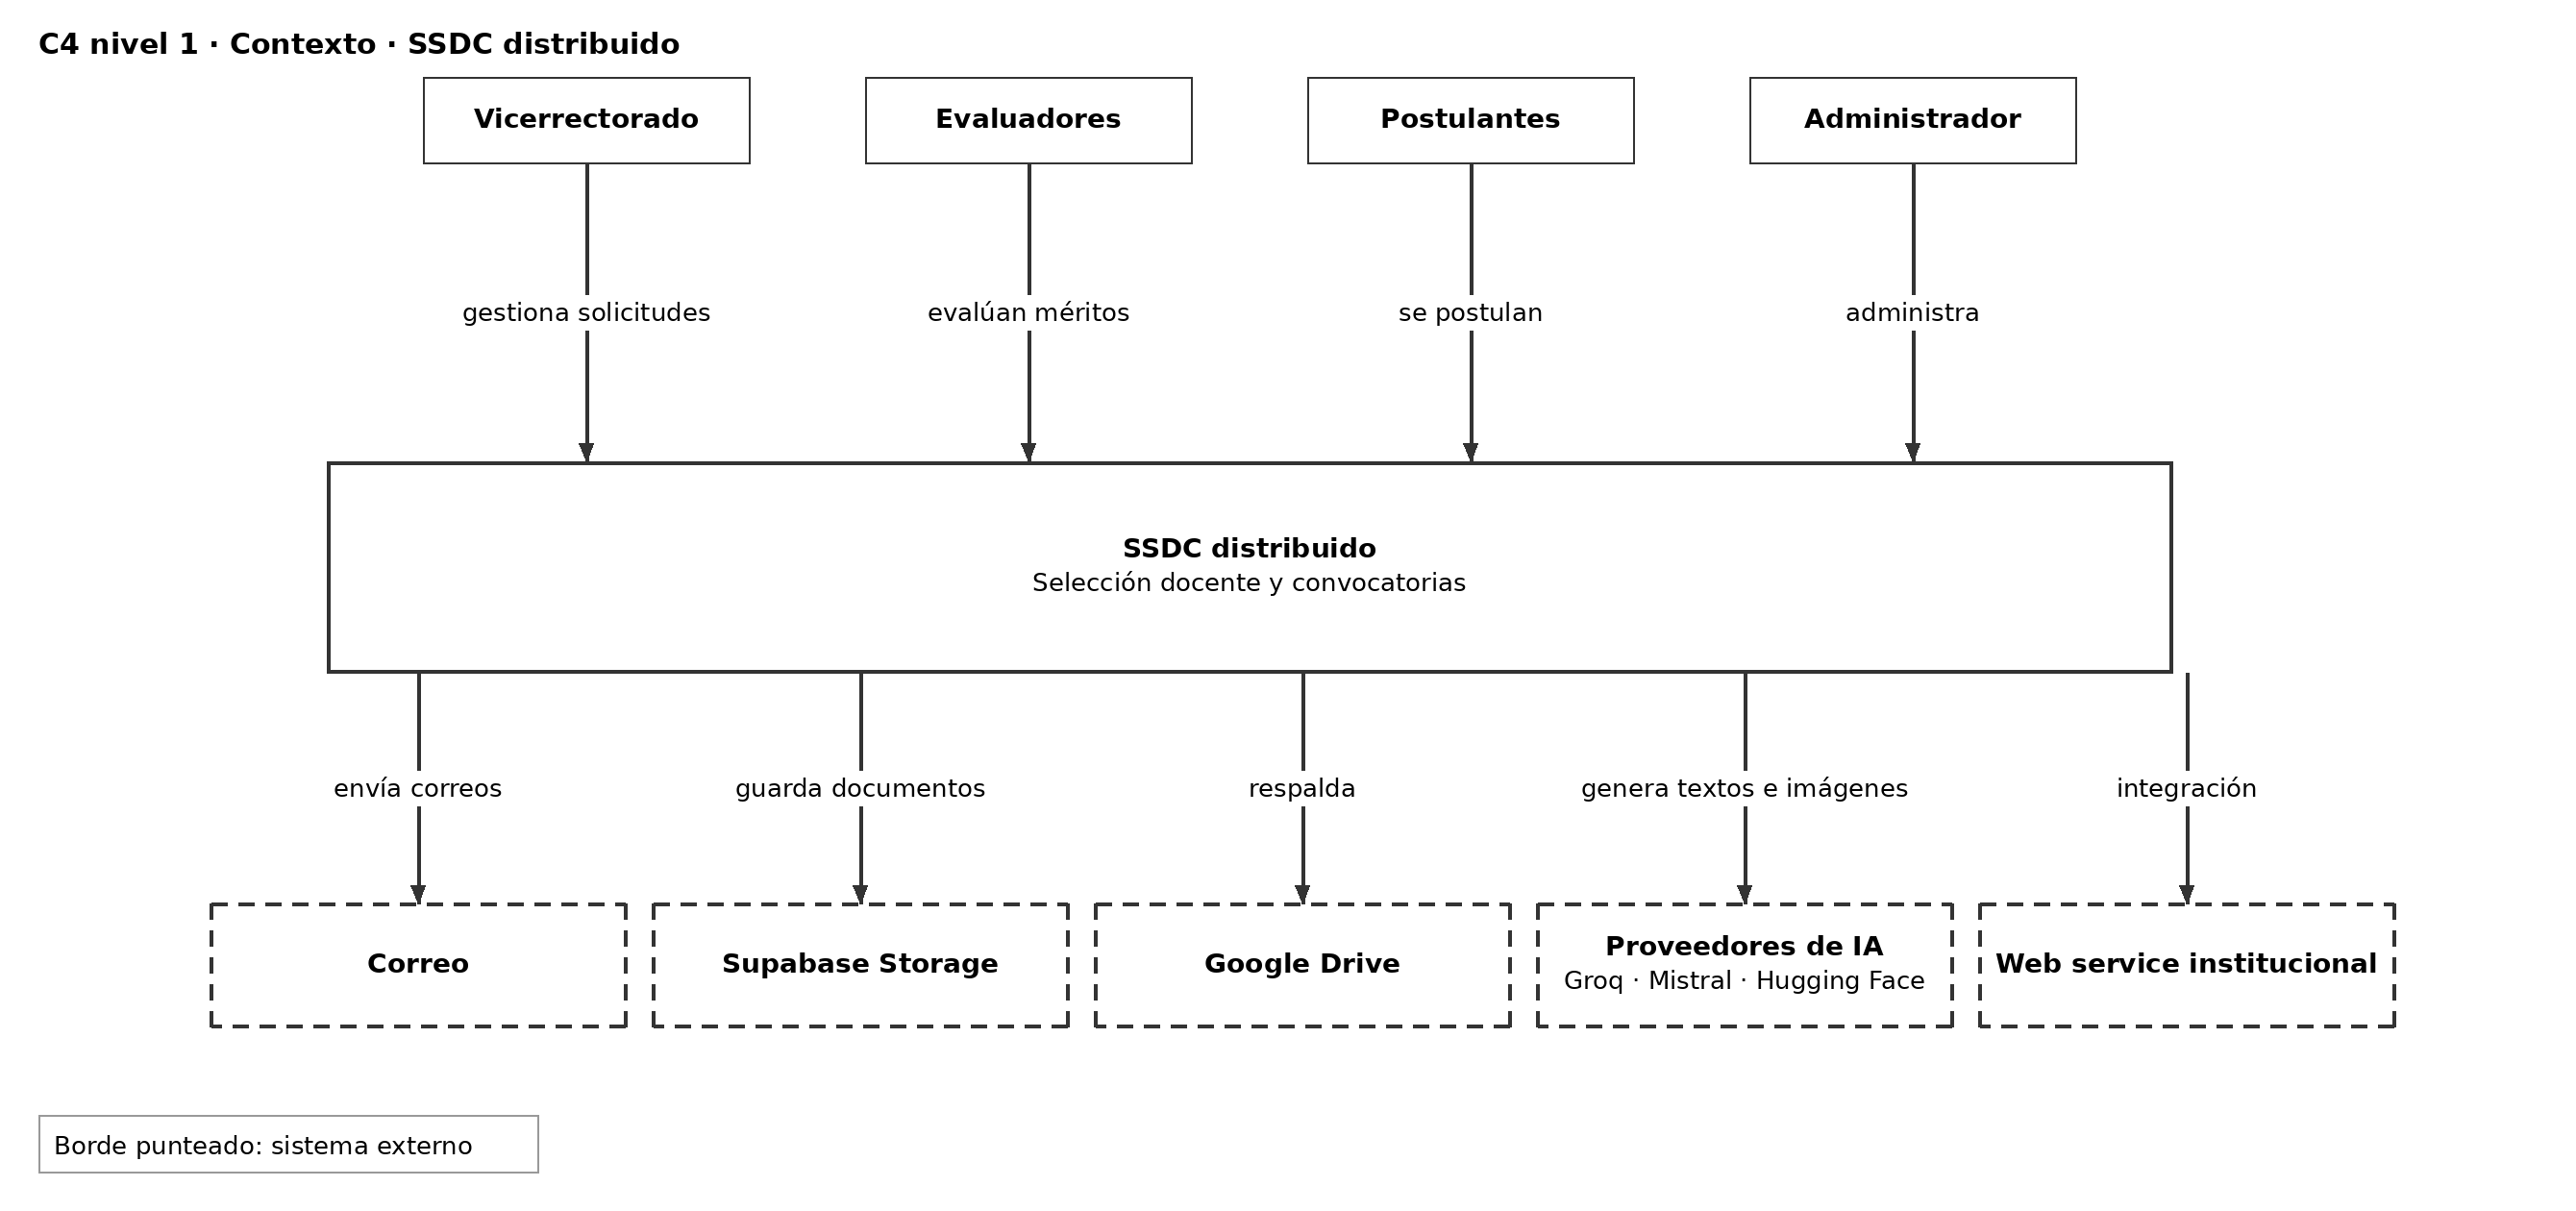
\includegraphics[width=0.93\textheight,angle=90]{c4-nivel1-contexto.png}
  \caption{C4 nivel 1: contexto del SSDC distribuido.}
\end{figure}

\subsection{Nivel 2: contenedores}

El diagrama de contenedores muestra un frontend, un API gateway que valida el token y seis servicios. Cuatro de ellos tienen su propia base PostgreSQL: postulaciones, evaluación, convocatorias y auditoría. \texttt{convocatorias} y \texttt{notificaciones} están implementados en el esqueleto de \texttt{src/} y se comunican por HTTP. Los otros cuatro servicios, el API gateway (que validaría el token) y la cola de mensajes están planeados; el uso de la cola lo define el ADR-002.

\begin{figure}[p]
  \centering
  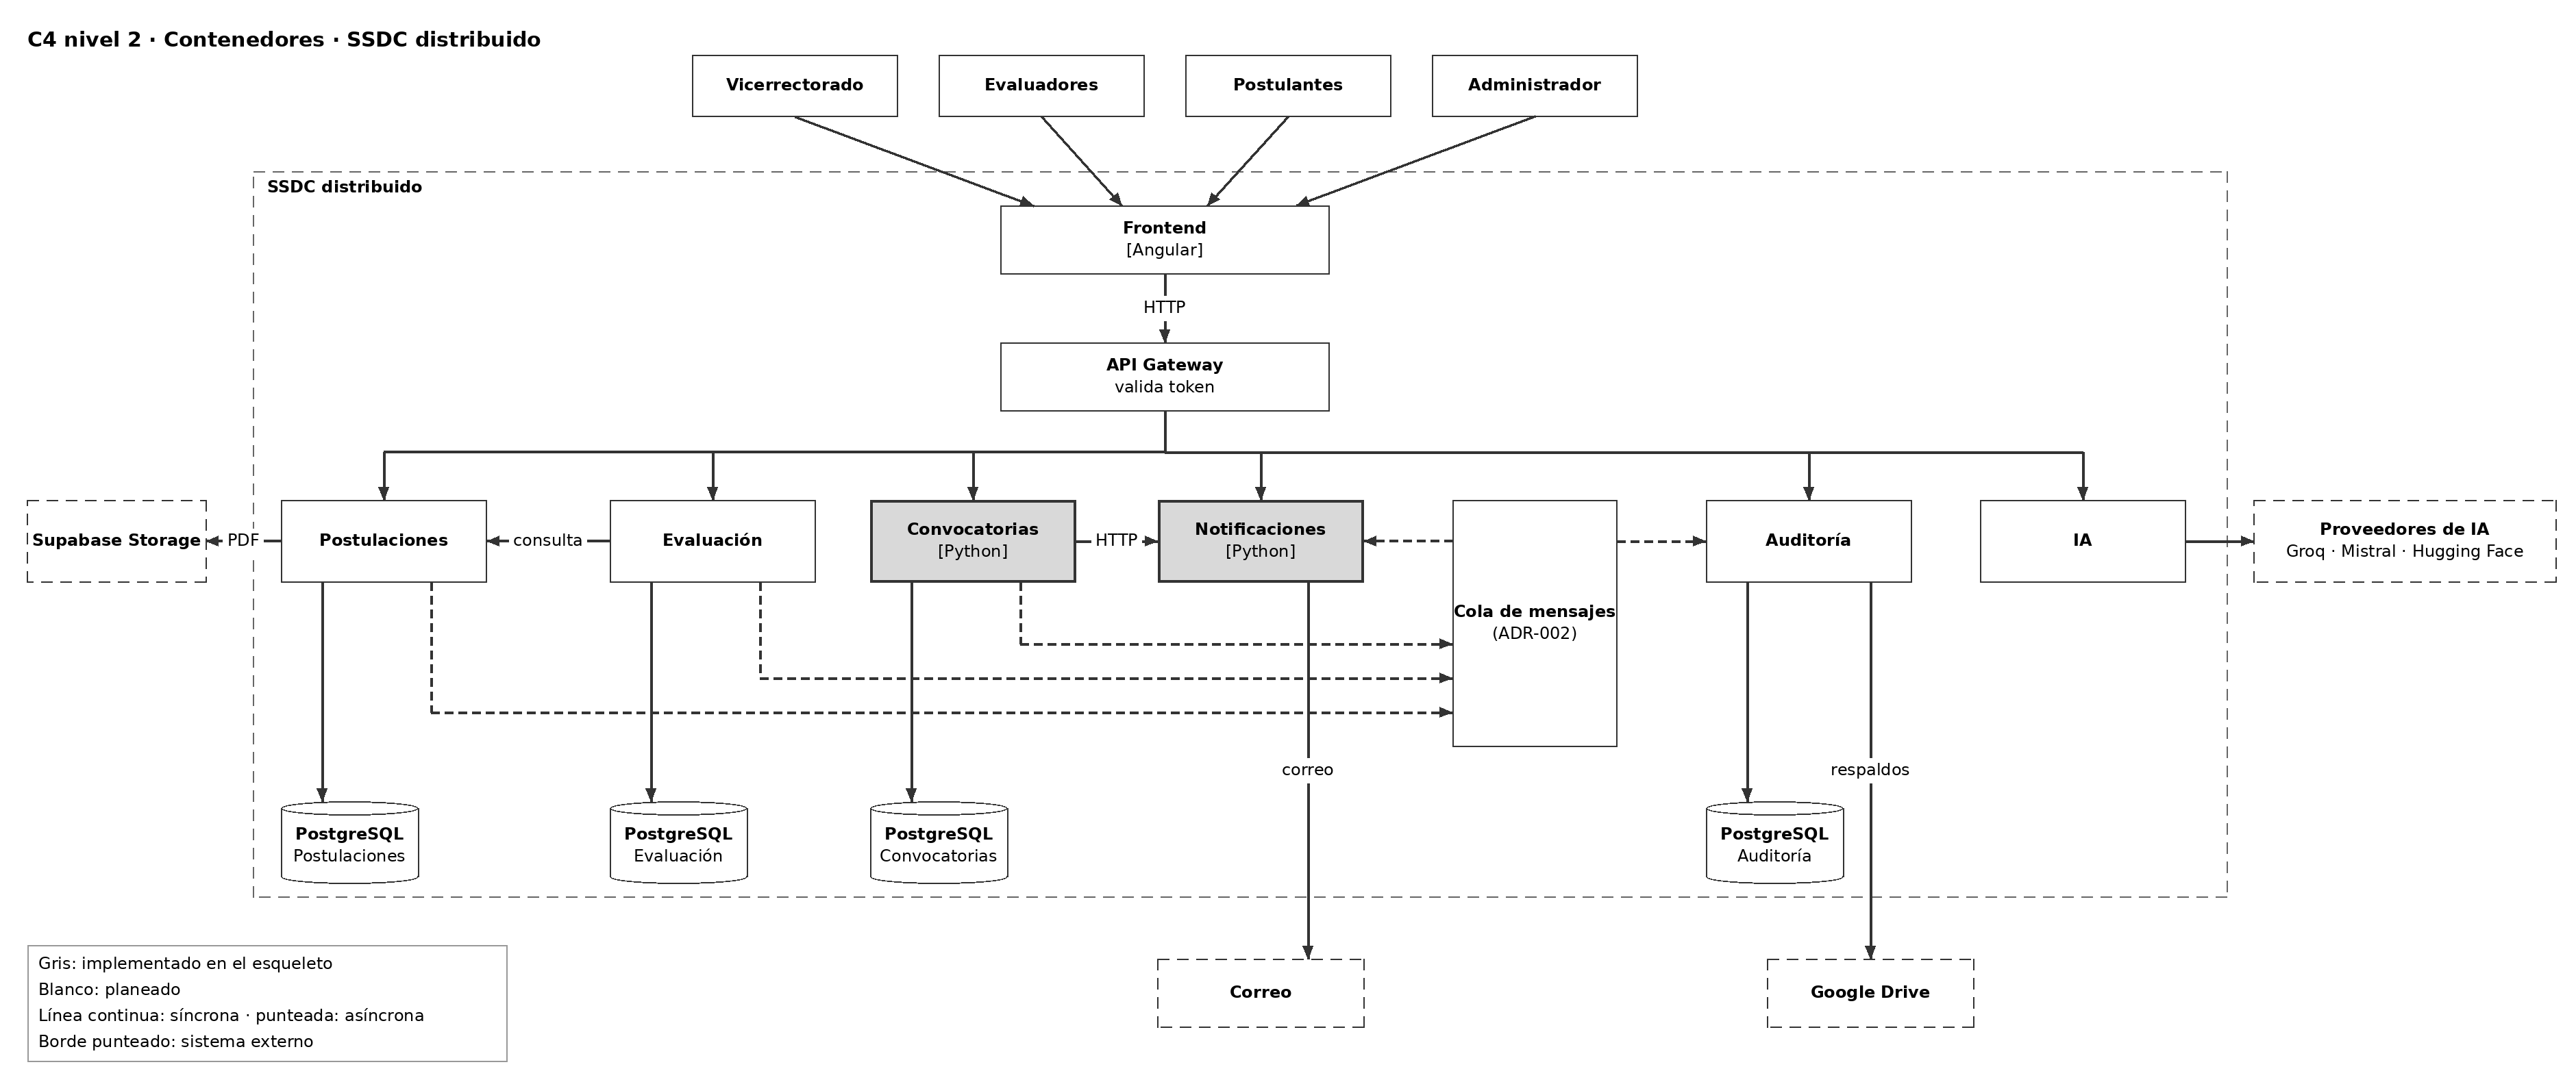
\includegraphics[width=0.93\textheight,angle=90]{c4-nivel2-contenedores.png}
  \caption{C4 nivel 2: contenedores del SSDC distribuido. En gris, los servicios implementados en el esqueleto.}
\end{figure}

\begin{table}[H]
\centering
\small
\caption{Contenedores del sistema}
\begin{tabularx}{\linewidth}{@{}p{3.1cm}p{2.7cm}X@{}}
\toprule
\textbf{Contenedor} & \textbf{Estado} & \textbf{Responsabilidad} \\
\midrule
\texttt{convocatorias} & esqueleto & Lista y publica convocatorias, y al publicar avisa a \texttt{notificaciones} por HTTP. Planeado: solicitudes docentes y creación de convocatorias. \\
\texttt{notificaciones} & esqueleto & Recibe avisos, los guarda en memoria y los lista. Planeado: envío del correo de cambio de estado. \\
\texttt{postulaciones} & planeado & Prepostulación, expediente en PDF (Supabase Storage) y estado de la postulación. \\
\texttt{evaluacion} & planeado & Matriz de méritos, ranking, entrevistas y clases demostrativas. Consulta a \texttt{postulaciones}. \\
\texttt{auditoria} & planeado & Registro de cambios con hash SHA-256 y respaldos hacia Google Drive. \\
\texttt{ia} & planeado & Generación asistida de textos e imágenes con proveedores externos. \\
\bottomrule
\end{tabularx}
\end{table}

\section{Modelo de comunicación entre servicios}
\emergencystretch=3em

Esta sección describe cómo se comunican los dos servicios del esqueleto que está en la carpeta \texttt{src/} del repositorio. No describe todavía el sistema completo: los nombres y puertos son provisionales hasta cerrar el ADR-002.

\subsection{Servicios del esqueleto}

\begin{table}[H]
\centering
\small
\caption{Servicios del esqueleto}
\begin{tabularx}{\linewidth}{@{}p{3.1cm}p{1.6cm}X@{}}
\toprule
\textbf{Servicio} & \textbf{Puerto} & \textbf{Responsabilidad} \\
\midrule
\texttt{convocatorias} & 8081 & Lista convocatorias de ejemplo y las publica. Al publicar una, avisa al otro servicio. \\
\texttt{notificaciones} & 8082 & Recibe avisos, los guarda en memoria y los lista. \\
\bottomrule
\end{tabularx}
\end{table}

\subsection{Mecanismo usado en esta entrega}

Los servicios se comunican por HTTP con mensajes en formato JSON. El servicio \texttt{convocatorias} actúa como cliente y \texttt{notificaciones} como servidor. Cuando se publica una convocatoria ocurre lo siguiente:

\begin{enumerate}[leftmargin=*]
  \item El cliente envía \texttt{POST /convocatorias/\{id\}/publicar} a \texttt{convocatorias}.
  \item \texttt{convocatorias} cambia el estado de la convocatoria a \emph{publicada}.
  \item \texttt{convocatorias} envía \texttt{POST /notificaciones} a \texttt{notificaciones} con el evento \texttt{ConvocatoriaPublicada}, el identificador y el título. Espera la respuesta como máximo 2 segundos.
  \item Si \texttt{notificaciones} responde, la respuesta de \texttt{convocatorias} incluye \texttt{notificacion: enviada}.
  \item Si \texttt{notificaciones} no responde, la respuesta incluye \texttt{notificacion: pendiente}. La convocatoria queda publicada y el servicio sigue atendiendo solicitudes.
\end{enumerate}

\subsection{Comportamiento observado}

Las pruebas se ejecutaron el 20 de noviembre de 2026 desde un clon limpio del repositorio, siguiendo el README de \texttt{src/}, en la máquina DESKTOP-H4C4SME. Las capturas están en la carpeta \texttt{evidencias/}.

\begin{table}[H]
\centering
\small
\caption{Resultados de las pruebas del esqueleto}
\begin{tabularx}{\linewidth}{@{}p{3.6cm}XX@{}}
\toprule
\textbf{Situación} & \textbf{Resultado observado} & \textbf{Evidencia} \\
\midrule
Ambos servicios activos & Los dos responden a \texttt{/health}. & \path|01-servicios-en-marcha.png| \\
Publicar la convocatoria 2 & Respuesta con \texttt{notificacion: enviada} y un aviso registrado en \texttt{notificaciones}. & \path|02-comunicacion-entre-servicios.png| \\
\texttt{notificaciones} detenido & Publicar la convocatoria 1 responde con \texttt{notificacion: pendiente}; \texttt{convocatorias} sigue activo. & \path|03-tolerancia-a-fallos.png| \\
\bottomrule
\end{tabularx}
\end{table}

\subsection{Interacciones del diagrama de contenedores}

La tabla recoge cada flecha del diagrama C4 de contenedores (nivel 2). \emph{Sinc.} es una llamada que espera respuesta y \emph{asinc.} deja un evento en la cola y sigue. De todo el diagrama, en el esqueleto solo está implementada la interacción de \texttt{convocatorias} con \texttt{notificaciones}, y hoy es HTTP directo; en el diagrama ese camino pasa por la cola, que es lo planeado según el ADR-002. El resto son decisiones de diseño sin implementar. Los usuarios (Vicerrectorado, Evaluadores, Postulantes y Administrador) usan el Frontend desde el navegador y no se listan como interacción entre contenedores.

{\small
\begin{longtable}{@{}p{3.7cm}p{1.3cm}p{2.9cm}p{5.6cm}@{}}
\caption{Interacciones entre contenedores y mecanismo propuesto}\\
\toprule
\textbf{Interacción} & \textbf{Tipo} & \textbf{Mecanismo} & \textbf{Justificación} \\
\midrule
\endfirsthead
\toprule
\textbf{Interacción} & \textbf{Tipo} & \textbf{Mecanismo} & \textbf{Justificación} \\
\midrule
\endhead
Frontend $\to$ API Gateway & Sinc. & HTTP con JSON & El usuario espera la respuesta en pantalla; el gateway valida el token antes de pasar la solicitud. \\
API Gateway $\to$ Postulaciones & Sinc. & HTTP con JSON & Consulta u orden que necesita respuesta inmediata, con tiempo máximo de espera. \\
API Gateway $\to$ Evaluación & Sinc. & HTTP con JSON & Igual que la anterior: el evaluador necesita ver el resultado. \\
API Gateway $\to$ Convocatorias & Sinc. & HTTP con JSON & Es el mecanismo que ya está probado en el esqueleto. \\
API Gateway $\to$ Auditoría & Sinc. & HTTP con JSON & Consulta de registros de auditoría por parte del Administrador. \\
API Gateway $\to$ Notificaciones & Sinc. & HTTP con JSON & Consulta de las notificaciones del usuario; es lectura, no aviso. \\
API Gateway $\to$ IA & Sinc. & HTTP con JSON & La persona espera el resultado del análisis; la llamada necesita tiempo máximo de espera. \\
Evaluación $\to$ Postulaciones & Sinc. & HTTP con JSON & Evaluación necesita los datos de la postulación para continuar (etiqueta \emph{consulta} del diagrama). \\
Postulaciones $\to$ Supabase Storage & Sinc. & API HTTP del servicio & Se guardan y leen los PDF de los documentos; hay que saber si la carga se completó. \\
Postulaciones $\to$ PostgreSQL & Sinc. & Conexión SQL & Cada servicio con datos tiene su propia base (ADR-001). \\
Evaluación $\to$ PostgreSQL & Sinc. & Conexión SQL & Igual: base propia por servicio. \\
Convocatorias $\to$ PostgreSQL & Sinc. & Conexión SQL & Igual: base propia por servicio. \\
Auditoría $\to$ PostgreSQL & Sinc. & Conexión SQL & Igual: base propia por servicio. \\
Convocatorias $\to$ Cola & Asinc. & Cola de mensajes (ADR-002) & Publica el evento de convocatoria publicada sin esperar a que el receptor esté disponible. \\
Evaluación $\to$ Cola & Asinc. & Cola de mensajes (ADR-002) & Publica el evento de evaluación terminada; el aviso tolera retraso. \\
Postulaciones $\to$ Cola & Asinc. & Cola de mensajes (ADR-002) & Publica el evento de postulación recibida; el aviso tolera retraso. \\
Cola $\to$ Auditoría & Asinc. & Cola de mensajes (ADR-002) & Auditoría consume los eventos cuando puede, con confirmación de recepción. \\
Cola $\to$ Notificaciones & Asinc. & Cola de mensajes (ADR-002) & Un aviso no se pierde si notificaciones está caído, que es la limitación del esqueleto. \\
Auditoría $\to$ Google Drive & Sinc. & API HTTP del servicio (respaldos) & Hay que confirmar que el respaldo se escribió. \\
Notificaciones $\to$ Correo & Sinc. & Protocolo del servicio de correo & El proveedor responde si aceptó el envío; el mecanismo exacto se define en E2. \\
IA $\to$ Proveedores de IA & Sinc. & API HTTP del proveedor & Los proveedores (Groq, Mistral, Hugging Face) se consumen por su API; hay que limitar el tiempo de espera. \\
\bottomrule
\end{longtable}
}

\subsection{Limitaciones conocidas}

\begin{itemize}[leftmargin=*]
  \item Los datos están en memoria; al reiniciar un servicio se pierden.
  \item Un aviso que queda \emph{pendiente} no se reintenta: si \texttt{notificaciones} vuelve a estar disponible, ese aviso no se envía solo.
  \item No hay autenticación entre servicios.
  \item La llamada es síncrona: \texttt{convocatorias} espera la respuesta (hasta 2 segundos) antes de contestar.
\end{itemize}

\subsection{Propuesta para el ADR-002}

La decisión definitiva del mecanismo se toma en el ADR-002 con el Arquitecto. Como punto de partida, se propone separar dos tipos de comunicación:

\begin{itemize}[leftmargin=*]
  \item \textbf{Consultas}, que necesitan respuesta inmediata: HTTP síncrono, con tiempo máximo de espera.
  \item \textbf{Avisos}, que toleran retraso, como las notificaciones: mensajería asíncrona con confirmación de recepción y cola de mensajes fallidos, de modo que un aviso no se pierda si el servicio receptor está caído.
\end{itemize}

Esta propuesta responde a la limitación del aviso \emph{pendiente} y se relaciona con el requisito RNF-04 (manejo de fallos). Está sin implementar: el esqueleto actual solo usa HTTP.

%\section{Análisis CAP y PACELC}

El teorema CAP permite analizar qué ocurre cuando una partición de red impide que partes de un sistema distribuido se comuniquen. Durante esa partición, no se puede garantizar al mismo tiempo la consistencia fuerte y que todas las solicitudes reciban una respuesta. PACELC amplía el análisis: cuando no hay partición, también considera el compromiso entre consistencia y latencia \cite{gilbert2002brewer,abadi2012pacelc}.

Este análisis se plantea para la arquitectura futura del SSDC, donde se proponen servicios separados y bases de datos propias. El esqueleto de esta entrega solo contiene los servicios \texttt{convocatorias} y \texttt{notificaciones}; guarda datos en memoria y no implementa réplicas ni pruebas de particiones. Por ello, las decisiones siguientes son propuestas de diseño, no propiedades ya implementadas o medidas.

\begin{table}[H]
\centering
\small
\caption{Propuesta de prioridades CAP y PACELC para datos críticos}
\begin{tabularx}{\linewidth}{@{}p{2.7cm}XXp{3.2cm}@{}}
\toprule
\textbf{Dato crítico} &
\textbf{Durante una partición (CAP)} &
\textbf{Sin partición (PACELC)} &
\textbf{Consecuencia para el usuario} \\
\midrule
Postulaciones y documentos &
Priorizar la consistencia. No confirmar una operación hasta verificar que quedó registrada en el servicio responsable. &
Priorizar la consistencia al confirmar escrituras, aunque la coordinación pueda aumentar la latencia. &
El envío puede quedar pendiente o rechazarse temporalmente; así se evita informar como guardado un expediente que no se confirmó. \\

Puntajes de evaluación &
Priorizar la consistencia. Suspender o diferir cambios si no se puede verificar el estado autorizado del puntaje. &
Priorizar la consistencia sobre la latencia al guardar una evaluación. &
El evaluador puede tener que reintentar, pero el sistema evita confirmar versiones contradictorias del puntaje. \\

Auditoría de cambios &
Priorizar la consistencia del registro. No presentar como auditado un cambio cuyo evento no se haya conservado de forma durable. &
Priorizar la consistencia y el orden del registro, aunque la confirmación tarde más. &
La operación puede demorarse o quedar pendiente mientras se registra el evento. Un hash por sí solo no garantiza que varias réplicas mantengan el mismo estado. \\

Notificaciones &
Priorizar la recepción del evento cuando pueda guardarse de forma durable; marcarlo como pendiente y enviarlo al recuperarse el servicio. &
Priorizar la latencia de la operación principal mediante envío asíncrono; el estado de la notificación puede actualizarse después. &
La operación principal puede continuar y el correo llegar con retraso. El sistema debe evitar anunciar que ya fue entregado si solo quedó pendiente. \\
\bottomrule
\end{tabularx}
\end{table}

Zhang et al. evaluaron mecanismos de disponibilidad y tolerancia a fallos en una arquitectura de microservicios \cite{zhang2025microservices}. Su estudio aporta una referencia para examinar la recuperación futura del SSDC, pero no verifica las prioridades CAP propuestas para este proyecto.

Estas prioridades son preliminares y deben revisarse con el Arquitecto antes de considerarlas decisiones definitivas. Para sostenerlas, el diseño tendrá que precisar cómo se confirman las escrituras, cómo se reintentan las solicitudes sin duplicarlas y cómo se conservan los eventos de auditoría y notificación cuando un servicio no está disponible.
\section{Registros de decisiones de arquitectura}

Los registros completos están en \texttt{docs/adr/}, en Markdown. Cada uno tiene contexto, opciones consideradas, decisión y consecuencias. Aquí se resumen.

\subsection{ADR-001: estilo de arquitectura}

\begin{description}[leftmargin=!,labelwidth=3.6cm,style=nextline]
  \item[Opciones] Monolito en capas (el actual), monolito modular y microservicios.
  \item[Decisión] Microservicios: un servicio por módulo del C4, y los que guardan datos tienen su propia base. En E1 se implementan dos.
  \item[Razón] Una dependencia externa caída afecta solo a un servicio (RNF-04), cada servicio se despliega sin reiniciar los demás, los programadores salen del proceso principal y un cambio de esquema afecta a un servicio (R4).
  \item[Consecuencia] Más procesos y red entre servicios, y datos repartidos en varias bases, lo que obliga al análisis CAP y PACELC.
\end{description}

\subsection{ADR-002: mecanismo de comunicación}

\begin{description}[leftmargin=!,labelwidth=3.6cm,style=nextline]
  \item[Opciones] HTTP síncrono con JSON, gRPC y mensajería asíncrona con cola.
  \item[Decisión] HTTP síncrono con tiempo máximo de espera para consultas y para el aviso del esqueleto actual. Cola de mensajes para los avisos de los servicios que se agreguen en E2, sin implementarla en E1.
  \item[Razón] Solo HTTP está implementado y probado en el esqueleto, y cuando \texttt{notificaciones} cae, \texttt{convocatorias} informa \emph{pendiente}, lo que cubre RNF-04 solo en parte. Los consumidores de la cola todavía no existen.
  \item[Consecuencia] Un aviso pendiente no se reenvía mientras no exista la cola, y la llamada síncrona retiene al emisor hasta 2 segundos.
\end{description}

\section{Análisis de riesgos}
% Fila R4 del análisis de riesgos (Eduardo Reinoso, Arquitecto).
% Se incluye desde 12_riesgos.tex con % Fila R4 del análisis de riesgos (Eduardo Reinoso, Arquitecto).
% Se incluye desde 12_riesgos.tex con % Fila R4 del análisis de riesgos (Eduardo Reinoso, Arquitecto).
% Se incluye desde 12_riesgos.tex con \input{secciones/12_riesgo_R4}
\subsection{R4: cambio de esquema aplicado sin revisión}

\begin{description}[leftmargin=!,labelwidth=4.2cm,style=nextline]
  \item[Incidente de origen]
    El 28 de febrero de 2017, en la región US-EAST-1, una persona del equipo de Amazon S3 ejecutó un comando para quitar unos pocos servidores del subsistema de facturación. Uno de los parámetros estaba mal escrito y el comando quitó muchos más, entre ellos servidores de los subsistemas de índice y de colocación. S3 dejó de atender solicitudes y tardó unas 4 h 17 min en volver a la normalidad\footnote{Informe de AWS sobre el evento: \url{https://aws.amazon.com/message/41926/}.}. Después, AWS hizo que la herramienta retire capacidad más despacio y le puso un mínimo por subsistema.
  \item[Relación con el SSDC]
    La herramienta aceptó una entrada equivocada y la ejecutó completa, sin un tope ni una confirmación. En CHRSweb el \texttt{application.properties} del backend tiene activa la línea \texttt{spring.jpa.hibernate.ddl-auto=update} (línea 56). Con ella, Hibernate crea o altera tablas y columnas al arrancar, según las entidades, y nadie revisa ese cambio antes. No borra columnas, pero si varios servicios comparten la base, el que arranque primero puede dejar un esquema distinto del que esperan los demás.
  \item[Probabilidad]
    Media: cada despliegue con entidades modificadas aplica el cambio.
  \item[Impacto]
    Alto: el cambio llegaría a las tablas de postulaciones y de puntajes.
  \item[Medida en E1]
    El esqueleto no tiene base de datos (guarda los datos en memoria), así que en E1 no hay un esquema que pueda cambiar. Cuando cada servicio tenga su base (E2), Hibernate quedará en modo de solo validación y los cambios de esquema se aplicarán con scripts versionados en el repositorio.
  \item[Verificación]
    En E2, con la base ya creada, se arranca un servicio con una entidad incompatible a propósito; debe negarse a iniciar y mostrar el error de validación. El resultado se anota en la bitácora.
\end{description}


% Riesgo R1 de Joseph Calderón, basado en el incidente de Cloudflare de 2022.
\subsection{R1: despliegue de una regla con alcance excesivo}

\begin{description}[leftmargin=!,labelwidth=4.2cm,style=nextline]
  \item[Incidente de origen]
    El 21 de junio de 2022, Cloudflare desplegó un cambio en sus políticas de anuncios de rutas BGP. El reordenamiento de términos hizo que se retiraran prefijos críticos y dejó fuera de servicio 19 centros de datos; el incidente afectó el 50\,\% de las solicitudes HTTP globales. Cloudflare indicó que las etapas del despliegue no fueron lo bastante pequeñas para detectar el problema antes de que alcanzara los centros afectados \cite{cloudflare2022outage}.

  \item[Relación con el SSDC]
    El backend actual concentra las funciones del SSDC. Un cambio incorrecto en la matriz de méritos o en las reglas de validación podría afectar varias convocatorias y postulaciones. En la arquitectura distribuida futura, un despliegue amplio de una regla compartida también podría propagar el error a más de un servicio.

  \item[Probabilidad]
    Media, como estimación cualitativa del equipo; no corresponde a una frecuencia medida.

  \item[Impacto]
    Alto: un error podría bloquear postulaciones o producir evaluaciones incorrectas durante una convocatoria.

  \item[Medida propuesta]
    El esqueleto de E1 no implementa la matriz de méritos, por lo que esta medida aún no está implementada. Para las siguientes etapas se propone versionar las reglas, exigir revisión antes de publicarlas, probarlas automáticamente y desplegarlas por etapas con una opción de reversión.

  \item[Verificación]
    En E1, dejar documentados estos controles como propuesta. Cuando se implemente la evaluación, probar una regla inválida y comprobar que las pruebas impidan publicarla; después, verificar en un despliegue controlado que una reversión restaure la versión anterior.
\end{description}
\subsection{R4: cambio de esquema aplicado sin revisión}

\begin{description}[leftmargin=!,labelwidth=4.2cm,style=nextline]
  \item[Incidente de origen]
    El 28 de febrero de 2017, en la región US-EAST-1, una persona del equipo de Amazon S3 ejecutó un comando para quitar unos pocos servidores del subsistema de facturación. Uno de los parámetros estaba mal escrito y el comando quitó muchos más, entre ellos servidores de los subsistemas de índice y de colocación. S3 dejó de atender solicitudes y tardó unas 4 h 17 min en volver a la normalidad\footnote{Informe de AWS sobre el evento: \url{https://aws.amazon.com/message/41926/}.}. Después, AWS hizo que la herramienta retire capacidad más despacio y le puso un mínimo por subsistema.
  \item[Relación con el SSDC]
    La herramienta aceptó una entrada equivocada y la ejecutó completa, sin un tope ni una confirmación. En CHRSweb el \texttt{application.properties} del backend tiene activa la línea \texttt{spring.jpa.hibernate.ddl-auto=update} (línea 56). Con ella, Hibernate crea o altera tablas y columnas al arrancar, según las entidades, y nadie revisa ese cambio antes. No borra columnas, pero si varios servicios comparten la base, el que arranque primero puede dejar un esquema distinto del que esperan los demás.
  \item[Probabilidad]
    Media: cada despliegue con entidades modificadas aplica el cambio.
  \item[Impacto]
    Alto: el cambio llegaría a las tablas de postulaciones y de puntajes.
  \item[Medida en E1]
    El esqueleto no tiene base de datos (guarda los datos en memoria), así que en E1 no hay un esquema que pueda cambiar. Cuando cada servicio tenga su base (E2), Hibernate quedará en modo de solo validación y los cambios de esquema se aplicarán con scripts versionados en el repositorio.
  \item[Verificación]
    En E2, con la base ya creada, se arranca un servicio con una entidad incompatible a propósito; debe negarse a iniciar y mostrar el error de validación. El resultado se anota en la bitácora.
\end{description}


% Riesgo R1 de Joseph Calderón, basado en el incidente de Cloudflare de 2022.
\subsection{R1: despliegue de una regla con alcance excesivo}

\begin{description}[leftmargin=!,labelwidth=4.2cm,style=nextline]
  \item[Incidente de origen]
    El 21 de junio de 2022, Cloudflare desplegó un cambio en sus políticas de anuncios de rutas BGP. El reordenamiento de términos hizo que se retiraran prefijos críticos y dejó fuera de servicio 19 centros de datos; el incidente afectó el 50\,\% de las solicitudes HTTP globales. Cloudflare indicó que las etapas del despliegue no fueron lo bastante pequeñas para detectar el problema antes de que alcanzara los centros afectados \cite{cloudflare2022outage}.

  \item[Relación con el SSDC]
    El backend actual concentra las funciones del SSDC. Un cambio incorrecto en la matriz de méritos o en las reglas de validación podría afectar varias convocatorias y postulaciones. En la arquitectura distribuida futura, un despliegue amplio de una regla compartida también podría propagar el error a más de un servicio.

  \item[Probabilidad]
    Media, como estimación cualitativa del equipo; no corresponde a una frecuencia medida.

  \item[Impacto]
    Alto: un error podría bloquear postulaciones o producir evaluaciones incorrectas durante una convocatoria.

  \item[Medida propuesta]
    El esqueleto de E1 no implementa la matriz de méritos, por lo que esta medida aún no está implementada. Para las siguientes etapas se propone versionar las reglas, exigir revisión antes de publicarlas, probarlas automáticamente y desplegarlas por etapas con una opción de reversión.

  \item[Verificación]
    En E1, dejar documentados estos controles como propuesta. Cuando se implemente la evaluación, probar una regla inválida y comprobar que las pruebas impidan publicarla; después, verificar en un despliegue controlado que una reversión restaure la versión anterior.
\end{description}
\subsection{R4: cambio de esquema aplicado sin revisión}

\begin{description}[leftmargin=!,labelwidth=4.2cm,style=nextline]
  \item[Incidente de origen]
    El 28 de febrero de 2017, en la región US-EAST-1, una persona del equipo de Amazon S3 ejecutó un comando para quitar unos pocos servidores del subsistema de facturación. Uno de los parámetros estaba mal escrito y el comando quitó muchos más, entre ellos servidores de los subsistemas de índice y de colocación. S3 dejó de atender solicitudes y tardó unas 4 h 17 min en volver a la normalidad\footnote{Informe de AWS sobre el evento: \url{https://aws.amazon.com/message/41926/}.}. Después, AWS hizo que la herramienta retire capacidad más despacio y le puso un mínimo por subsistema.
  \item[Relación con el SSDC]
    La herramienta aceptó una entrada equivocada y la ejecutó completa, sin un tope ni una confirmación. En CHRSweb el \texttt{application.properties} del backend tiene activa la línea \texttt{spring.jpa.hibernate.ddl-auto=update} (línea 56). Con ella, Hibernate crea o altera tablas y columnas al arrancar, según las entidades, y nadie revisa ese cambio antes. No borra columnas, pero si varios servicios comparten la base, el que arranque primero puede dejar un esquema distinto del que esperan los demás.
  \item[Probabilidad]
    Media: cada despliegue con entidades modificadas aplica el cambio.
  \item[Impacto]
    Alto: el cambio llegaría a las tablas de postulaciones y de puntajes.
  \item[Medida en E1]
    El esqueleto no tiene base de datos (guarda los datos en memoria), así que en E1 no hay un esquema que pueda cambiar. Cuando cada servicio tenga su base (E2), Hibernate quedará en modo de solo validación y los cambios de esquema se aplicarán con scripts versionados en el repositorio.
  \item[Verificación]
    En E2, con la base ya creada, se arranca un servicio con una entidad incompatible a propósito; debe negarse a iniciar y mostrar el error de validación. El resultado se anota en la bitácora.
\end{description}


% Riesgo R1 de Joseph Calderón, basado en el incidente de Cloudflare de 2022.
\subsection{R1: despliegue de una regla con alcance excesivo}

\begin{description}[leftmargin=!,labelwidth=4.2cm,style=nextline]
  \item[Incidente de origen]
    El 21 de junio de 2022, Cloudflare desplegó un cambio en sus políticas de anuncios de rutas BGP. El reordenamiento de términos hizo que se retiraran prefijos críticos y dejó fuera de servicio 19 centros de datos; el incidente afectó el 50\,\% de las solicitudes HTTP globales. Cloudflare indicó que las etapas del despliegue no fueron lo bastante pequeñas para detectar el problema antes de que alcanzara los centros afectados \cite{cloudflare2022outage}.

  \item[Relación con el SSDC]
    El backend actual concentra las funciones del SSDC. Un cambio incorrecto en la matriz de méritos o en las reglas de validación podría afectar varias convocatorias y postulaciones. En la arquitectura distribuida futura, un despliegue amplio de una regla compartida también podría propagar el error a más de un servicio.

  \item[Probabilidad]
    Media, como estimación cualitativa del equipo; no corresponde a una frecuencia medida.

  \item[Impacto]
    Alto: un error podría bloquear postulaciones o producir evaluaciones incorrectas durante una convocatoria.

  \item[Medida propuesta]
    El esqueleto de E1 no implementa la matriz de méritos, por lo que esta medida aún no está implementada. Para las siguientes etapas se propone versionar las reglas, exigir revisión antes de publicarlas, probarlas automáticamente y desplegarlas por etapas con una opción de reversión.

  \item[Verificación]
    En E1, dejar documentados estos controles como propuesta. Cuando se implemente la evaluación, probar una regla inválida y comprobar que las pruebas impidan publicarla; después, verificar en un despliegue controlado que una reversión restaure la versión anterior.
\end{description}
\section{Plan del proyecto}

\subsection{Roles}
\begin{table}[H]
\centering
\caption{Roles del equipo CHRS}
\begin{tabularx}{\linewidth}{@{}p{4.2cm}p{3.6cm}X@{}}
\toprule
\textbf{Integrante} & \textbf{Rol} & \textbf{Responsabilidades} \\
\midrule
Silva Triviño John Jairo & Líder de Desarrollo & Repositorio, esqueleto en \texttt{/src}, modelo de comunicación, tablero e issues, video. \\
Herrera Barco Humberto Aldair & Responsable de Documentación & Documento \LaTeX, referencias, bitácora, compilación y PDF del SGA. \\
Reinoso Vélez Eduardo David & Arquitecto & Diagramas C4, justificación de la arquitectura y ADR. \\
Calderón Saltos Joseph & Responsable de Calidad & Requisitos no funcionales, CAP/PACELC, riesgos y pruebas del esqueleto. \\
\bottomrule
\end{tabularx}
\end{table}

\subsection{Tablero e issues}
El trabajo se organiza en el tablero \textit{PFC CHRS} de GitHub Projects, con las columnas
\textit{Por hacer}, \textit{En curso} y \textit{Hecho}. Cada issue tiene un responsable y la
etiqueta de su entrega (E1 o E2), y se cierra con un commit de quien lo realizó.

\subsection{Cronograma}
\begin{table}[H]
\centering
\caption{Cronograma de las entregas del PFC}
\begin{tabularx}{\linewidth}{@{}p{1.2cm}p{1.6cm}X@{}}
\toprule
\textbf{Entrega} & \textbf{Semana} & \textbf{Contenido} \\
\midrule
E1 & 5  & Definición, requisitos y arquitectura base \\
E2 & 9  & Microservicios, API y contenedores \\
E3 & 13 & Base de datos distribuida y procesamiento \\
E4 & 17 & Sistema final en capas, calidad, pruebas y defensa \\
\bottomrule
\end{tabularx}
\end{table}

%\section{Aportes individuales y uso de IA}

\subsection{Reinoso Vélez Eduardo David (Arquitecto)}

\begin{table}[H]
\centering
\small
\caption{Aportes de Eduardo Reinoso Vélez}
\begin{tabularx}{\linewidth}{@{}p{5.2cm}X@{}}
\toprule
\textbf{Entregable} & \textbf{Ubicación en el repositorio} \\
\midrule
Bosquejo a mano de la arquitectura & \texttt{evidencias/bosquejo-arquitectura-1-2026-11-20.jpg} \\
Diagrama C4 de contexto (nivel 1) & \texttt{docs/diagramas/c4-nivel1-contexto.*} \\
Diagrama C4 de contenedores (nivel 2) & \texttt{docs/diagramas/c4-nivel2-contenedores.*} \\
ADR-001 (estilo de arquitectura) & \texttt{docs/adr/ADR-001.md} \\
ADR-002 (comunicación entre servicios) & \texttt{docs/adr/ADR-002.md} \\
Plantilla de ADR & \texttt{docs/adr/PLANTILLA-ADR.md} \\
Secciones 07, 08, 11 y riesgo R4 & \texttt{docs/secciones/} \\
\bottomrule
\end{tabularx}
\end{table}

\paragraph{Herramienta.} Claude (Anthropic), modelo Sonnet 5.5, en la aplicación web y en una sesión conectada a la carpeta del repositorio.

\paragraph{Para qué se usó.} Proponer una estructura inicial a partir de la cual Eduardo dibujó el bosquejo a mano. Redactar los borradores de los ADR, de las secciones 07, 08 y 11 y de la fila de riesgo R4, que Eduardo revisó y ajustó. Generar los archivos \texttt{.drawio} de los diagramas C4.

\paragraph{Cómo se verificó.} Las cifras de CHRSweb (324 archivos Java, 52 controladores, la propiedad \texttt{ddl-auto} con valor \texttt{update} en la línea 56 de \texttt{application\allowbreak .properties}) se contaron en el código. El comportamiento del esqueleto se contrastó con \texttt{src/} y con las capturas de \texttt{evidencias/}. El documento se compiló sin errores. Eduardo revisó cada archivo antes de subirlo.


% ============================== REFERENCIAS ============================
\printbibliography[heading=bibintoc,title={Referencias}]

\end{document}
